
\documentclass[border=8pt, multi, tikz]{standalone} 
\usepackage{import}
\subimport{C:/Users/ahnd6/OneDrive/����/GitHub/Cell-counting/docs/plot_neural_net/layers/}{init}
\usetikzlibrary{positioning}
\usetikzlibrary{3d} %for including external image 

\def\ConvColor{rgb:yellow,5;red,2.5;white,5}
\def\ConvReluColor{rgb:yellow,5;red,5;white,5}
\def\PoolColor{rgb:red,1;black,0.3}
\def\UnpoolColor{rgb:blue,2;green,1;black,0.3}
\def\FcColor{rgb:blue,5;red,2.5;white,5}
\def\FcReluColor{rgb:blue,5;red,5;white,4}
\def\SoftmaxColor{rgb:magenta,5;black,7}   
\def\SumColor{rgb:blue,5;green,15}

\newcommand{\copymidarrow}{\tikz \draw[-Stealth,line width=0.8mm,draw={rgb:blue,4;red,1;green,1;black,3}] (-0.3,0) -- ++(0.3,0);}

\begin{document}
\begin{tikzpicture}
\tikzstyle{connection}=[ultra thick,every node/.style={sloped,allow upside down},draw=\edgecolor,opacity=0.7]
\tikzstyle{copyconnection}=[ultra thick,every node/.style={sloped,allow upside down},draw={rgb:blue,4;red,1;green,1;black,3},opacity=0.7]

\node[canvas is zy plane at x=0] (input) at (-5,0,0) {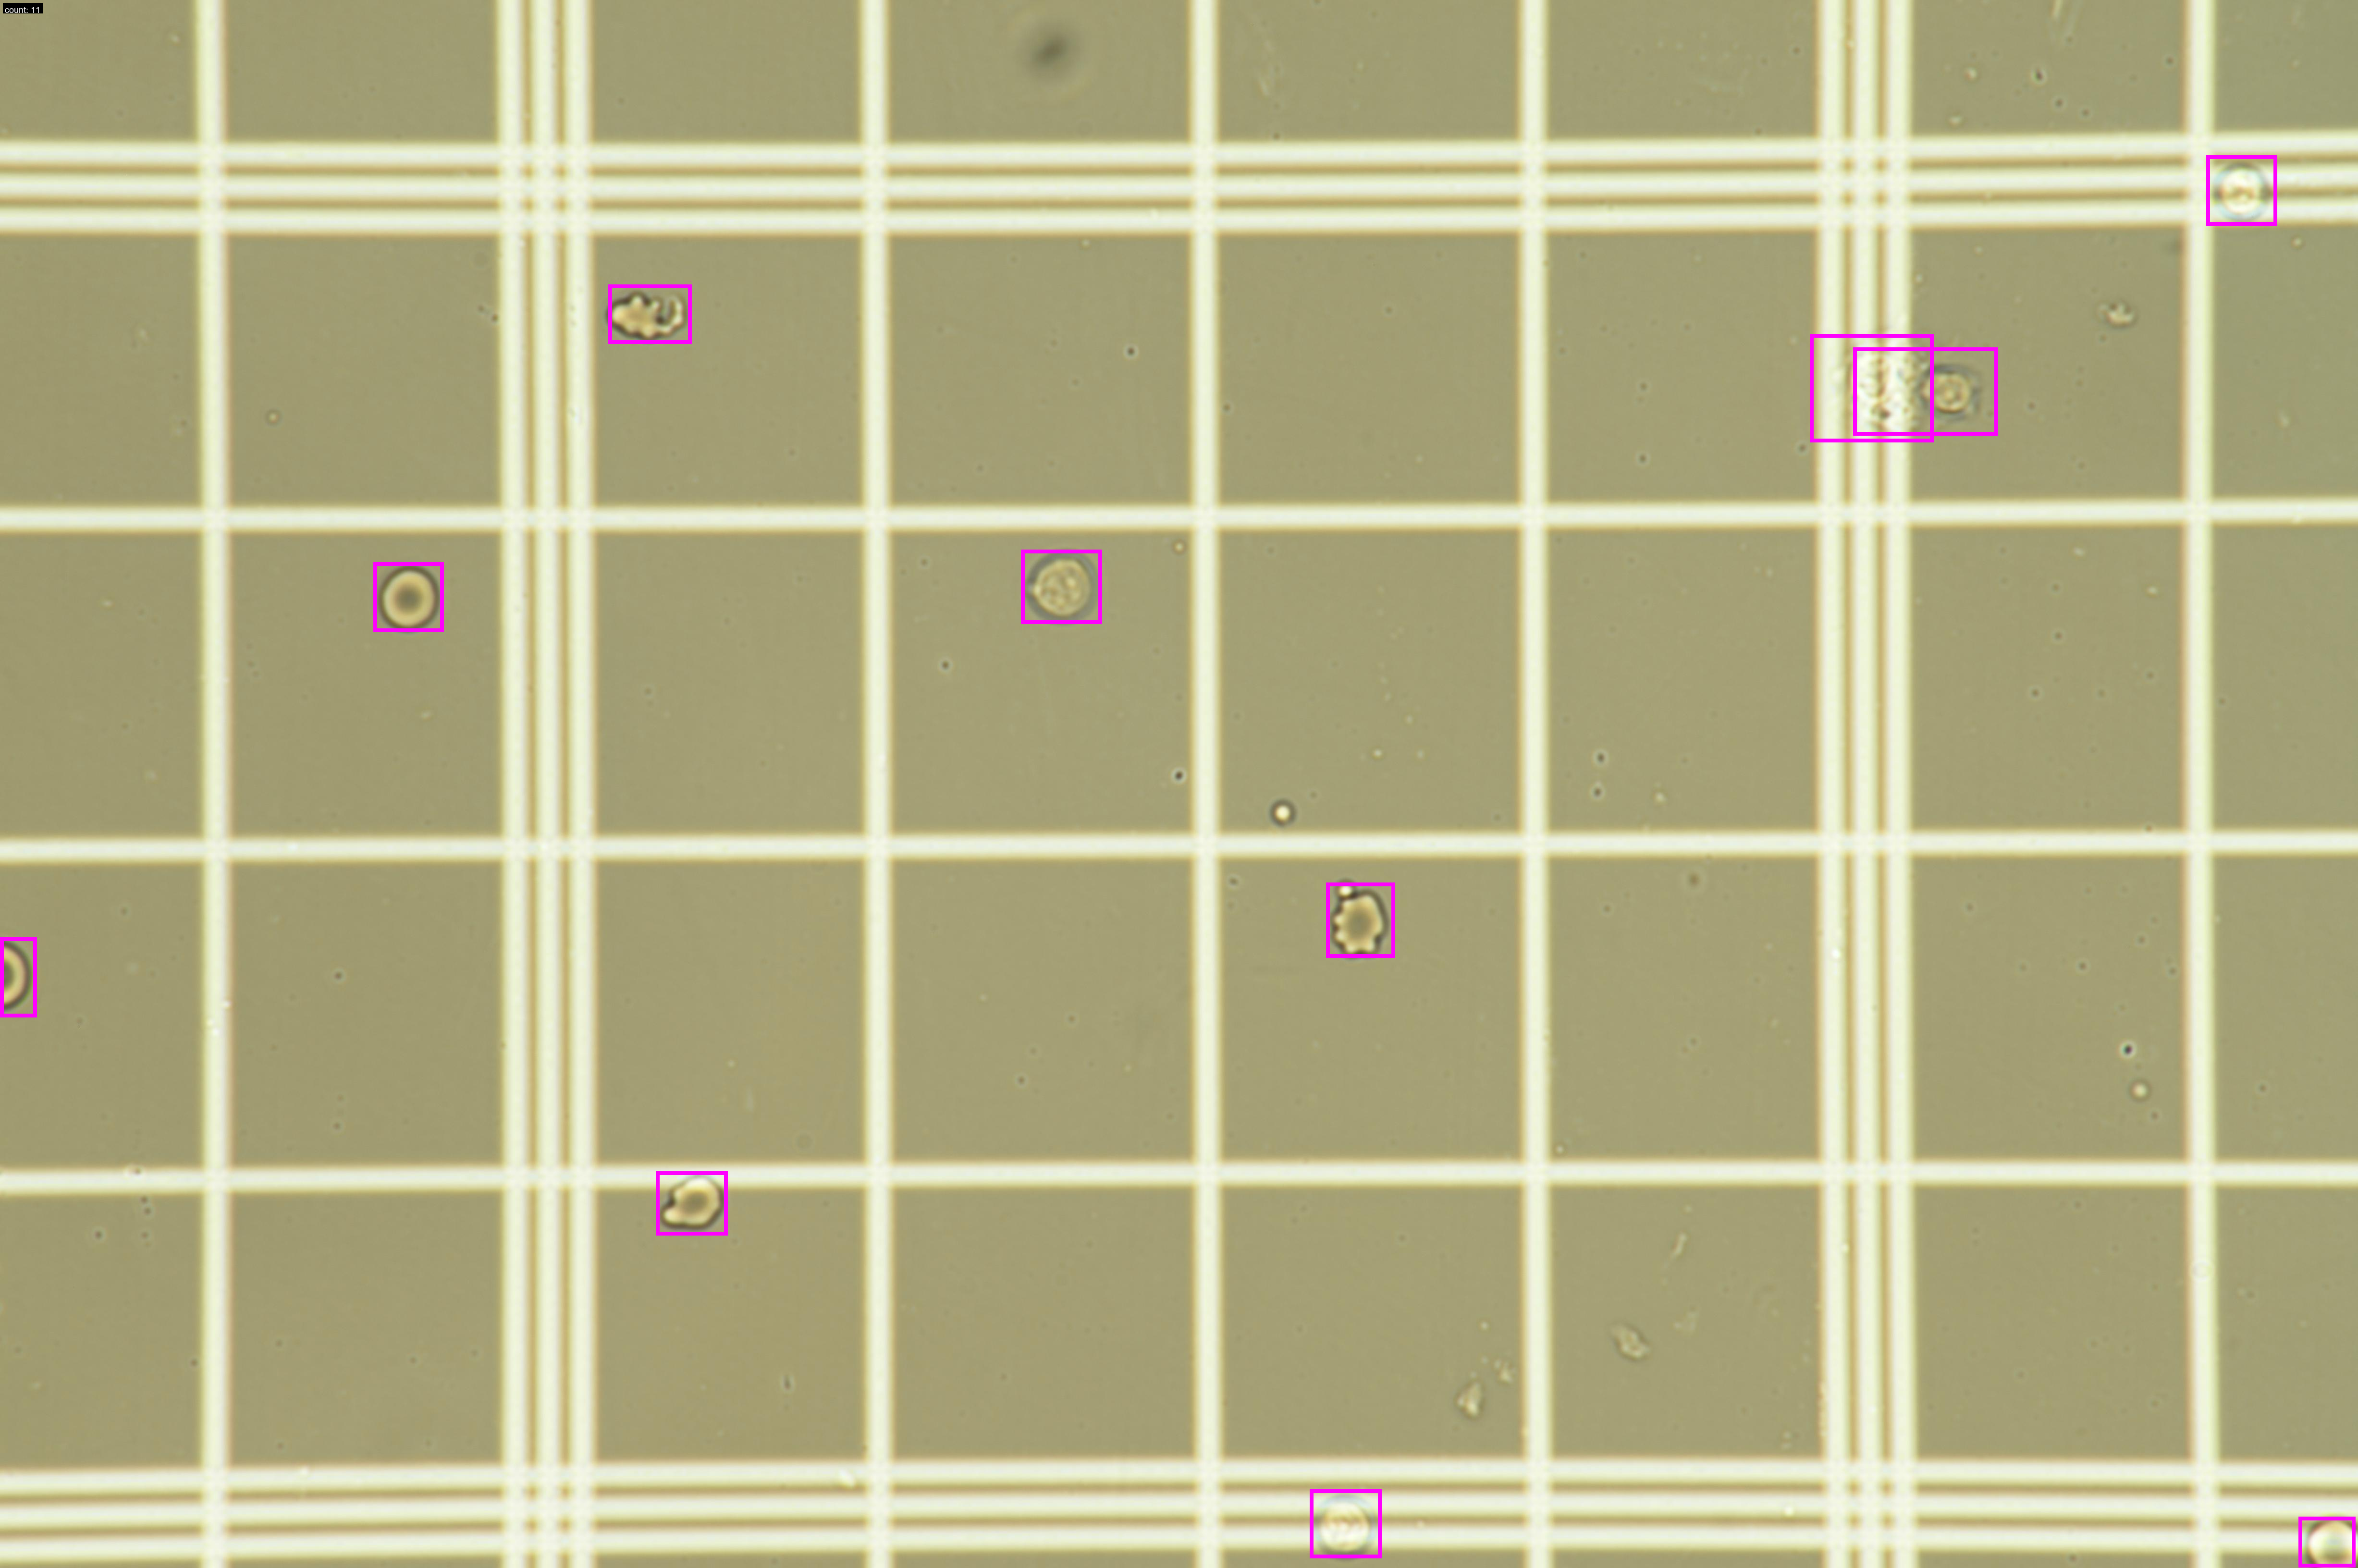
\includegraphics[width=5cm,height=5cm]{C:/Users/ahnd6/OneDrive/����/GitHub/Cell-counting/docs/assets/cell_counting_result.png}};

\pic[shift={(0,0,0)}] at (0,0,0) 
    {Box={
        name=stem,
        caption=Stem 7x7 Conv,
        xlabel={{64, }},
        zlabel=640,
        fill=\ConvColor,
        height=28,
        width=1.5,
        depth=28
        }
    };

\draw [connection]  (input-east)    -- node {\midarrow} (stem-west);

\pic[shift={(0,0,0)}] at (2,0,0) 
    {Box={
        name=c2,
        caption=ResNet C2,
        xlabel={{256, }},
        zlabel=320,
        fill=\ConvColor,
        height=24,
        width=2.5,
        depth=24
        }
    };

\draw [connection]  (stem-east)    -- node {\midarrow} (c2-west);

\pic[shift={(0,0,0)}] at (4.5,0,0) 
    {Box={
        name=c3,
        caption=ResNet C3,
        xlabel={{512, }},
        zlabel=160,
        fill=\ConvColor,
        height=20,
        width=3,
        depth=20
        }
    };

\draw [connection]  (c2-east)    -- node {\midarrow} (c3-west);

\pic[shift={(0,0,0)}] at (7.5,0,0) 
    {Box={
        name=c4,
        caption=ResNet C4,
        xlabel={{1024, }},
        zlabel=80,
        fill=\ConvColor,
        height=16,
        width=3.2,
        depth=16
        }
    };

\draw [connection]  (c3-east)    -- node {\midarrow} (c4-west);

\pic[shift={(0,0,0)}] at (10.5,0,0) 
    {Box={
        name=c5,
        caption=ResNet C5,
        xlabel={{2048, }},
        zlabel=40,
        fill=\ConvColor,
        height=12,
        width=3.4,
        depth=12
        }
    };

\draw [connection]  (c4-east)    -- node {\midarrow} (c5-west);

\pic[shift={(0,0,0)}] at (4.5,3,0) 
    {Box={
        name=p3,
        caption=FPN P3,
        xlabel={{256, }},
        zlabel=80,
        fill=\ConvColor,
        height=10,
        width=1.2,
        depth=10
        }
    };

\pic[shift={(0,0,0)}] at (7.5,3,0) 
    {Box={
        name=p4,
        caption=FPN P4,
        xlabel={{256, }},
        zlabel=40,
        fill=\ConvColor,
        height=9,
        width=1.2,
        depth=9
        }
    };

\pic[shift={(0,0,0)}] at (10.5,3,0) 
    {Box={
        name=p5,
        caption=FPN P5,
        xlabel={{256, }},
        zlabel=20,
        fill=\ConvColor,
        height=8,
        width=1.2,
        depth=8
        }
    };

\pic[shift={(0,0,0)}] at (13.5,3,0) 
    {Box={
        name=p6,
        caption=FPN P6,
        xlabel={{256, }},
        zlabel=10,
        fill=\ConvColor,
        height=7,
        width=1.2,
        depth=7
        }
    };

\pic[shift={(0,0,0)}] at (16.5,3,0) 
    {Box={
        name=p7,
        caption=FPN P7,
        xlabel={{256, }},
        zlabel=5,
        fill=\ConvColor,
        height=6,
        width=1.2,
        depth=6
        }
    };

\draw [connection]  (c3-east)    -- node {\midarrow} (p3-west);

\draw [connection]  (c4-east)    -- node {\midarrow} (p4-west);

\draw [connection]  (c5-east)    -- node {\midarrow} (p5-west);

\pic[shift={(0,0,0)}] at (19,1.5,0) 
    {Box={
        name=cls_head,
        caption=Classification Subnet,
        xlabel={{256, }},
        zlabel=9,
        fill=\ConvColor,
        height=9,
        width=1.2,
        depth=9
        }
    };

\draw [connection]  (p7-east)    -- node {\midarrow} (cls_head-west);

\pic[shift={(0,0,0)}] at (19,-1.5,0) 
    {Box={
        name=reg_head,
        caption=Regression Subnet,
        xlabel={{256, }},
        zlabel=9,
        fill=\ConvColor,
        height=9,
        width=1.2,
        depth=9
        }
    };

\draw [connection]  (p7-east)    -- node {\midarrow} (reg_head-west);

\pic[shift={(0,0,0)}] at (22,1.5,0) 
    {Box={
        name=detections,
        caption=Detections,
        xlabel={{" ","dummy"}},
        zlabel=2,
        fill=\SoftmaxColor,
        opacity=0.8,
        height=6,
        width=0.7,
        depth=6
        }
    };

\draw [connection]  (cls_head-east)    -- node {\midarrow} (detections-west);

\end{tikzpicture}
\end{document}
